%!TEX root = ../../main.tex

\toggletrue{image}
\toggletrue{imagehover}
\chapterimage{installing}
\chapterimagetitle{\uppercase{Installing}}
\chapterimageurl{https://xkcd.com/1367/}
\chapterimagehover{\tiny But still, my scheme for creating and saving user config files and data locally to preserve them across reinstalls might be useful for--wait, that's cookies.}

\chapter{Mit \acs{PHP} auf eine Datenbank zugreifen}
\label{chapter-php-datenbanken-zugreifen}

Mit \ac{PHP} können wir sehr einfach mit einem \ac{DBMS} kommunizieren. Insbesondere ist \ac{PHP} für eine breite Unterstützung von relationalen \ac{DBMS} bekannt. Wir müssen also nichts installieren und können direkt mit \ac{PHP} loslegen. Wir schauen uns in diesem Kapitel zunächst an, wie wir uns mit einem relationalen \ac{DBMS} verbinden können (z.B. MariaDB). Anschliessend besprechen wir den \ac{PHP}-Code, um einen \ac{SQL}-Befehl einbetten zu können. Die Lernziele lauten:

\newcommand{\mitPhpAufEineDatenbankZugreifenLernziele}{
\protect\begin{todolist}
\item Sie bauen mit \ac{PHP} die Verbindung zu einem relationalen \ac{DBMS} auf.
\item Sie fügen einen \lstinline[language=sql]{insert into}-Befehl (\ac{SQL}) in einen \ac{PHP}-Abschnitt ein.
\item Sie fügen einen \lstinline[language=sql]{select}-Befehl (\ac{SQL}) in einen \ac{PHP}-Abschnitt ein.
\end{todolist}
}

\lernziel{\autoref{chapter-php-datenbanken-zugreifen}, \nameref{chapter-php-datenbanken-zugreifen}}{\protect\mitPhpAufEineDatenbankZugreifenLernziele}

\mitPhpAufEineDatenbankZugreifenLernziele

\section{Konzept}

Mit \ac{PHP} schicken wir \ac{SQL}-Befehle an ein \ac{RDBMS}. Das Einfügen von Daten läuft wie folgt ab:

\begin{enumerate}
\item Mit dem \ac{DBMS} verbinden: \lstinline[language=PHP]{mysqli_connect(host, user, password, database name)}.
\item \lstinline[language=SQL]{insert into}-Befehl mit den Daten in einer Variablen speichern (z.B. \lstinline[language=PHP]{$sql}).
\item \ac{SQL}-Befehl an das \ac{DBMS} schicken: \lstinline[language=PHP]{mysqli_query(connection, query)}.
\item \ac{DBMS}-Verbindung schliessen: \lstinline[language=PHP]{mysqli_close(connection)}.
\end{enumerate}

\section{Beispiel: Daten einfügen}
\label{sec-beispiel-daten-einfuegen-sql-php}

Wir gehen hier davon aus, dass eine Tabelle mit dem \ac{SQL}-Befehl aus \autoref{lst-create-table-anmeldung} \textbf{zuvor} erstellt wurde. Es handelt sich um ein verkürztes Beispiel mit weniger Formulardaten (siehe \autoref{figure-formular-anmeldung-kompakt})

\begin{figure}[htb]
\begin{minipage}{0.45\textwidth}
\centering
\begin{lstlisting}[language=SQL, basicstyle=\ttfamily\tiny, morekeywords={text, real}, caption={\protect\acs{SQL}-Befehl zur Erstellung der Tabelle \texttt{anmeldung}.}, label={lst-create-table-anmeldung}]
create table anmeldung (
  vorname text,
  tour text,
  anzahl int,
  email text,
  passwort text
);
\end{lstlisting}
\end{minipage}
\hfill
\begin{minipage}{0.45\textwidth}
\centering
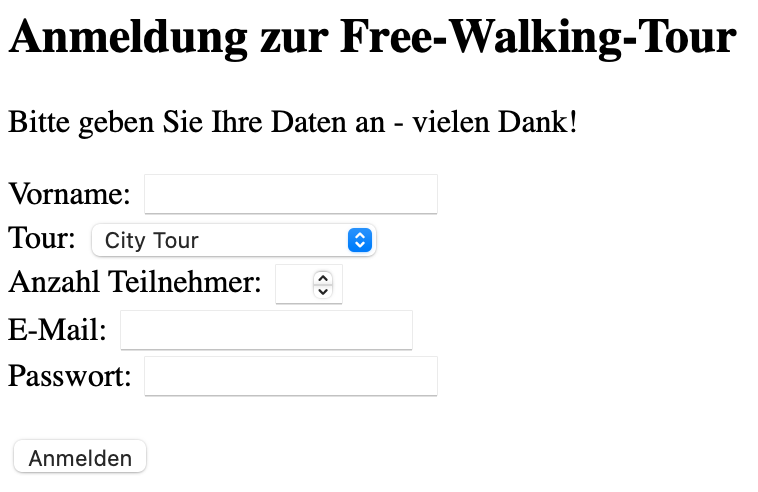
\includegraphics[scale=0.25]{formular.png}
\caption{Formular zur Anmeldung.}
\label{figure-formular-anmeldung-kompakt}
\end{minipage}
\end{figure}

Die Datenbanktabelle soll die Anmeldungen zu einer Free-Walking-Tour speichern. \autoref{lst-php-insert-into} zeigt den Inhalt der \ac{PHP}-Datei, welche aufgerufen wird, wenn das Formular abgeschickt wird. 

\subsection{Verbindungsaufbau}

Die \ac{PHP}-Datei in \autoref{lst-php-insert-into} beinhaltet in den ersten Zeilen (Zeile \num{1} bis Zeile \num{8}) die Verbindung zum \ac{DBMS}. Hier müssen wir die Verbindungsdaten angeben. Für den \lstinline{host} muss man typischerweise die Adresse zum \ac{DBMS} angeben.

\subsection{Formulardaten auslesen}

Im zweiten \ac{PHP}-Abschnitt werden in den Zeilen \num{18} bis \num{22} die Formulardaten ausgelesen (siehe \autoref{chapter-formulare-php}) und in Variablen gespeichert.

\subsection{Abfrage formulieren und abschicken}

Der zweite \ac{PHP}-Abschnitt beinhalten die Zeilen \num{24} bis \num{26} die \ac{PHP}-Funktionen zur Verarbeitung des \ac{SQL}-Befehls. In Zeile \num{24} wird der passende \lstinline[language=SQL]{insert into}-Befehl als \ac{PHP}-String notiert. Der String beinhaltet die Variablen mit den Formulardaten. Mit  \lstinline[language=PHP]{mysqli_query($verbindung, $sql)} wird der \ac{SQL}-Befehl an das \ac{DBMS} geschickt. Das Ergebnis des Befehls wird in der Variablen \lstinline[language=PHP]{$ergebnis} gespeichert. Das Ergebnis von \lstinline{mysql_query} beinhaltet bei einem  \lstinline[language=SQL]{insert into}-Befehl  die Anzahl der eingefügten Zeilen. Danach (Zeile 26) wird die Verbindung zum \ac{DBMS} geschlossen.

\subsection{Abfrageergebnis verarbeiten}

In den Zeilen \num{29} bis \num{33} wir das Abfrageergebnis benutzt. Die Variable \lstinline[language=PHP]{$ergebnis} beinhaltet die Anzahl der eingefügten Zeilen. Falls die Zeile erfolgreich in die Datenbank eingefügt werden konnte, dann speichert die Variable die Zahl \num{1}, sonst \num{0}. Dies wird durch die \lstinline[language=PHP]{if}-Bedingung geprüft. Die Ausgabe mit \lstinline[language=PHP]{echo} erfolgt also nur dann, wenn die Zeile erfolgreich eingefügt wurde.

\subsection{Ausgabe der Formulardaten}

Nach den Befehlen für die Kommunikation mit dem \ac{DBMS} folgt die Ausgabe der Formulardaten. Für jede Benutzereingabe gibt es einen Listeneintrag (\lstinline[language=HTML]{li}-Element). Darin gibt es einen kurzen \ac{PHP}-Abschnitt, welcher mit \lstinline[language=PHP]{echo} die Formulareingabe ausgibt. Diese \ac{PHP}-Abschnitte sind für die Kommunikation zum \ac{DBMS} \textbf{nicht} relevant.

\begin{lstlisting}[language=PHP, alsolanguage=HTML, upquote=true, caption={Anmeldedaten werden in der Tabelle \texttt{anmeldung} gespeichert.}, label={lst-php-insert-into}]
<?php
$verbindung = mysqli_connect(
  "code-yard.org",
  "dbu_22_alice",
  "superSecret",
  "db_22_alice"
);
?>
<!DOCTYPE html>
<html lang="de">
<head>
  <meta charset="UTF-8">
  <title>Feedback</title>
</head>
<body>
<h1>Feedback</h1>
<?php
$vorname = $_POST["vorname"];
$tour = $_POST["tour"];
$anzahl = $_POST["anzahl"];
$email = $_POST["email"];
$passwort = $_POST["passwort"];

$sql = "insert into anmeldung (vorname, tour, anzahl, 
email, passwort) values ('$vorname', '$tour', $anzahl, 
'$email', '$passwort')";
$ergebnis = mysqli_query($verbindung, $sql);
mysqli_close($verbindung);
if ($ergebnis == 1) {
  echo "<p>";
  echo "Anmeldung in der Datenbank gespeichert.";
  echo "</p>";
}
?>
<ul>
  <li>Vorname:<?php echo $vorname; ?></li>
  <li>Tour:<?php echo $tour; ?></li>
  <li>Anzahl Personen:<?php echo $anzahl; ?></li>
  <li>E-Mail-Adresse:<?php echo $email; ?></li>
  <li>Passwort:<?php echo $passwort; ?></li>
</ul>
</body>
</html>
?>
\end{lstlisting}

\begin{important}
Beim Formulieren von \ac{SQL}-Befehlen mit \ac{PHP} müssen wir auf die \textbf{korrekte Verwendung} der \textbf{Anführungszeichen} achten. Möchten wir in eine Spalte einen Text einfügen, dann müssen wir ein \textbf{einfaches} Anführungszeichen verwenden. Der \textbf{gesamte} \ac{SQL}-Befehl muss in \ac{PHP} jedoch in einem String gespeichert werden. Dazu benötigen wir \textbf{doppelte} Anführungszeichen.
\end{important}

\begin{example}
Zwei Beispiele zeigen die Verwendung der Anführungszeichen.

\begin{lstlisting}[language=PHP, upquote=true]
$sql = "insert into person (vorname, nachname, alter) 
values ('Alice', 'Cooper', 42)";
\end{lstlisting}

\begin{lstlisting}[language=PHP, upquote=true]
$vorname = "Alice";
$sql = "insert into person (vorname, nachname, alter) 
values ('$vorname', 'Cooper', 42)";
\end{lstlisting}

\end{example}

\section{Wo ist der \acs{PHP}-Code für das Erstellen der Tabelle?}

Eine Tabelle wird typischerweise ohne \ac{PHP} erstellt. Das Erstellen der Tabelle ist (meistens) ein \textbf{einmaliger} Vorgang. Meist verbindet man sich \textbf{direkt} mit dem \ac{DBMS} (Query Console) und führt den \lstinline[language=SQL]{create table}-Befehl aus. Gezielt dafür ein \ac{PHP}-Skript zu erstellen ist ein unnötiger Aufwand, aber natürlich möglich. Gibt es einmal eine Änderung an der Tabelle (z.B. eine zusätzliche Spalte), dann kann man auch dies direkt über die Query Console erledigen.

\newpage

\section{Beispiel: Daten ausgeben}

Wir gehen bei diesem Beispiel davon aus, dass das Beispiel aus \autoref{sec-beispiel-daten-einfuegen-sql-php} vorhanden ist und einige Zeilen in die Datenbanktabelle eingefügt wurden. Wir möchten nun mit einer \ac{PHP}-Datei alle Anmeldungen anzeigen. \autoref{lst-php-select-from-beispiel} zeigt dazu ein vollständiges Beispiel. Die ersten Zeilen sind recht ähnlich zum Einfügen von Daten. Wir gehen deshalb hier nur auf die neuen \ac{PHP}-Codezeilen ein. Die neuen Codezeilen umfassen die Zeilen \num{24} bis \num{38}.

\begin{lstlisting}[language=PHP, alsolanguage=HTML, upquote=true, caption={Alle Anmeldedaten aus der Tabelle \texttt{anmeldung} werden auf der Webseite angezeigt.}, label={lst-php-select-from-beispiel}]
<?php
$verbindung = mysqli_connect(
  "code-yard.org",
  "dbu_22_alice",
  "superSecret",
  "db_22_alice"
);
?>
<!DOCTYPE html>
<html lang="de">
<head>
  <meta charset="UTF-8">
  <title>Admin</title>
</head>
<body>
<h1>Admin</h1>
<p>
 Liste der Anmeldungen:
</p>
<?php
$sql = "select vorname, tour, anzahl, email, passwort 
from anmeldung";
$ergebnis = mysqli_query($verbindung, $sql);
while ($zeile = mysqli_fetch_row($ergebnis)) {
  $vorname = $zeile[0];
  $tour = $zeile[1];
  $anzahl = $zeile[2];
  $email = $zeile[3];
  $passwort = $zeile[4];
  echo "<ul>";
  echo "<li>Vorname: $vorname</li>";
  echo "<li>Tour: $tour</li>";
  echo "<li>Anzahl Teilnehmer: $anzahl</li>";
  echo "<li>E-Mail: $email</li>";
  echo "<li>Passwort: $passwort</li>";
  echo "</ul>";
  echo "<hr>";
}
mysqli_close($verbindung);
?>
</body>
</html>
\end{lstlisting}

\subsection{Abfrageergebnis verarbeiten}

Das Ergebnis des \lstinline[language=SQL]{select}-Befehls beinhaltet nun eine Tabelle. Wir können die Tabelle jedoch nicht auf einmal ausgeben, sondern müssen \textbf{Zeile für Zeile} der Tabelle verarbeiten. Dies wird über eine \lstinline[language=PHP]{while}-Schleife in Kombination mit \lstinline[language=PHP]{mysqli_fetch_row} erledigt. Der \ac{PHP}-Befehl \lstinline[language=PHP]{mysqli_fetch_row} sorgt dafür, dass \textbf{eine Zeile nach der anderen Zeile} in der Variablen \lstinline[language=PHP]{$zeile} gespeichert wird. Der Körper der \lstinline[language=PHP]{while}-Schleife wird dann \textbf{pro Zeile} einmal ausgeführt. Innerhalb der \lstinline[language=PHP]{while}-Schleife können wir dann die Spalten auslesen. Jede Spalte besitzt eine Nummer, den sogenannten Index. Mithilfe der eckigen Klammern und dem Index können wir auf eine Spalte zugreifen und den Wert auslesen. Der Index wird durch die Reihenfolge der Spalten im \lstinline[language=SQL]{select}-Befehl festgelegt. Bei der Abfrage aus dem Beispiel wäre dies wie folgt:

\begin{lstlisting}[language=SQL, mathescape, numbers=none]

select $\smash{\overbrace{\texttt{vorname}}^{0}}$, $\smash{\overbrace{\texttt{tour}}^{1}}$, $\smash{\overbrace{\texttt{anzahl}}^{2}}$, $\smash{\overbrace{\texttt{email}}^{3}}$, $\smash{\overbrace{\texttt{passwort}}^{4}}$ 
from anmeldung
\end{lstlisting}